\chapter{Proposta}
Nos estudos realizados por \citeonline{Canfora2014} e \citeonline{Hassan:2009:PFU:1555001.1555024} foram analisados a relação da entropia de mudança com a qualidade do projeto e algumas métricas de software, como por exemplo, número de contribuidores, no entanto, várias métricas não foram analisadas nesses estudos e não há uma ferramenta que monitore a entropia, métricas sociais, de autoria e de processo.

Portanto o objetivo é implementar uma ferramenta que monitore o valor da entropia de mudança e sua relação com as métricas sociais, de autoria e de processo dos projetos. A ferramenta terá seis módulos que serão apresentados a seguir:

\begin{figure}[h]
	\captionsetup{justification=centering}
	\includegraphics[width=\linewidth]{fluxogramaTCC.png}
	\caption{Fluxograma do funcionamento da ferramenta}
	\label{figura:fluxogramaimagem}
\end{figure}

\section{Coletar dados}
O módulo de coleta de dados é responsável pela extração de dados dos projetos do Github e Git que serão persistidos em um banco de dados local. Os dados serão obtidos utilizando o GHTorrent\footnote{GHTorrent é uma ferramenta que monitora os eventos públicos do Github, para cada evento é armazenado o seu conteúdo e as resposta JSON são armazenadas em um banco de dados MongoDB e também no MySQL} e a API Github.

Utilizando a base de dados MySQL do GHTorrent será extraído dados sobre os \textit{commits}, \textit{issues}, \textit{Pull Requests} e contribuidores do projeto. Além disso, será feito o clone das versões do projeto selecionado utilizando o comando \textit{git log}, \textit{git clone} e \textit{git reset}. 

\section{Calcular entropia}
Este módulo que realiza o cálculo da entropia de cada arquivo do projeto no período que o usuário informar. O valor da entropia será determinado utilizando como medida o número de commits que o arquivo teve durante um período de tempo selecionado pelo usuário. Para o cálculo da entropia é necessário medir a diferença da métrica Revisões(número total de commits) gerada pela ferramenta Change Metrics entre duas versões diferentes do projeto e assim obter o número de commits que cada arquivo teve entre uma versão e outra.

\section{Calcular métricas}
O módulo de cálculo das métricas irá realizar o cálculo após a extração dos dados no módulo de coleta de dados. Nessa etapa o usuário deverá informar quais métricas ele deseja calcular e uma data anterior a data atual. O período definido será entre a data atual e a data definida pelo usuário e as métricas serão calculadas de 15 em 15 dias.

Para o cálculo das métrica de processo será utilizada a ferramenta Change Metrics e para executá-la é necessário passar três parâmetros: o projeto git, o arquivo csv onde serão armazenados os dados e tipo do projeto que pode ser \textit{all} ou \textit{single}. O comando para executar a Change Metrics é: java -jar <tool.jar> projeto arquivo.csv single. 

A forma como as métricas serão calculadas estão descritas na tabela 3.1. 

\begin{table}[H]
\centering
\caption{Tabela de cálculo das métricas}
\label{cálculometricas}
\begin{tabular}{|p{3cm}|p{12cm}|}
\hline
Métrica                             & Descrição do cálculo                                                                        \\ \hline
Authorship                          & Média da quantidade de commits considerando todos os contribuidores                         \\ \hline
Ownership                           & Maior valor da métrica de authorship                                                        \\ \hline
Experiência                         & Média da quantidade de linhas modificadas no arquivo por todos os contribuidores            \\ \hline
Pull Request fechados por arquivo   & Contagem do número de Pull Request fechados relacionados a um determinado arquivo           \\ \hline
Pull Request abertos por arquivo    & Contagem do número de Pull Request abertos relacionados a um determinado arquivo            \\ \hline
Comentários em Pull Request aberto  & Contagem do número de comentários em todos os Pull Request abertos relacionados ao arquivo  \\ \hline
Comentários em Pull Request fechado & Contagem do número de comentários em todos os Pull Request fechados relacionados ao arquivo \\ \hline
Quantidade de commits               & Calculado utilizando a ferramenta Change Metrics                                        \\ \hline
Quantidade de defeitos              & Calculado utilizando a ferramenta Change Metrics                                            \\ \hline
Idade do arquivo                    & Calculado utilizando a ferramenta Change Metrics                                            \\ \hline
Quantidade de linhas removidas      & Calculado utilizando a ferramenta Change Metrics                                            \\ \hline
Quantidade de linhas adicionadas    & Calculado utilizando a ferramenta Change Metrics                                            \\ \hline
Code Churn                          & Calculado utilizando a ferramenta Change Metrics                                            \\ \hline
Quantidade de refatorações          & Calculado utilizando a ferramenta Change Metrics                                            \\ \hline
Max Change set                      & Calculado utilizando a ferramenta Change Metrics                                            \\ \hline
Average Change set                  & Calculado utilizando a ferramenta Change Metrics                                            \\ \hline
\end{tabular}
\end{table}

\section{Gerar relatório de análise estatística}
Como foi feito na pesquisa de \citeonline{Canfora2014}, para analisar a relação da entropia e as métricas de software serão utilizados os métodos estatísticos de \textit{Wilcoxon}, \textit{ANOVA} e \textit{Cliff's Delta}, onde todos os testes serão feitos no ambiente estístico R com nível de significância de 95\%.

O teste de \textit{Wilcoxon} pareado é um método não-paramétrico para comparação de duas amostras com o objetivo de verificar se existem diferenças significativas entre elas. E para mensurar a diferença entre as amostras é utilizado o \textit{Cliff's Delta}, uma medida de tamanho de efeito não-paramétrico, por exemplo, pode ser utilizada para mensurar a diferença no valor da entropia de mudança antes e depois da refatoração.

O \textit{ANOVA} (Análise de Variância) é usada para verificar se a média de duas ou mais populações são iguais e determina se as diferenças entre as médias amostrais sugerem diferenças significativas entre as médias das populações ou se essas diferenças decorrem apenas da variabilidade ímplicita de cada amostra. O método \textit{ANOVA} irá ser utilizado para analisar a interação entre a entropia de mudança e outras métricas de software. 

Após a análise estatísticas será gerado um relatório informando o usuário identificando quais métricas apresentam maior relação com a entropia e quais arquivos possuem maior entropia.

\section{Gerar Visualização}
Este módulo permite o usuário utilizar filtros para escolher quais métricas ele deseja visualizar. Para visualização será utilizado o \textit{Treemapping}, \textit{Heat Map} e gráficos de duas dimensões.

O treemapping é uma forma de visualização de dados de forma hierárquica utilizando retângulos aninhados. Na ferramenta o \textit{Treemapping} será utilizado para visualizar o valor da entropia dos arquivos do projeto, onde cada retângulo representará um arquivo e o tamanho desse retângulo representa o valor da entropia, quanto maior a entropia maior será o retângulo. O usuário poderá escolher qual período de tempo ele deseja visualizar o valor da entropia e também poderá comparar esse valor entre dois peŕiodos diferentes, sendo que o valor da entropia é calculado de 15 em 15 dias.

\begin{figure}[H]
	\captionsetup{justification=centering}
	\centerline{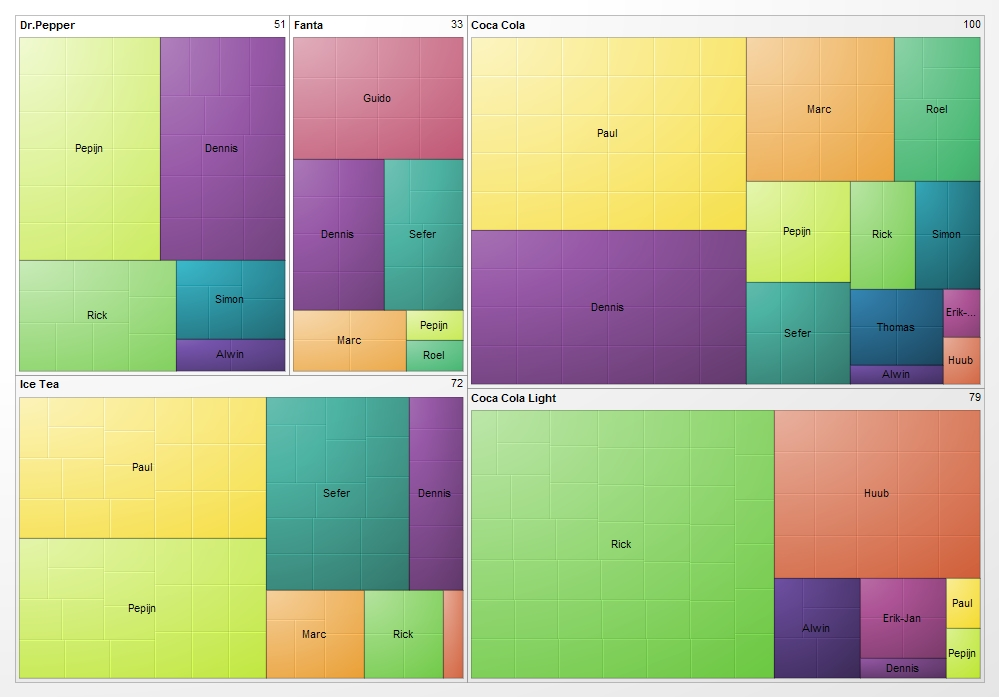
\includegraphics[scale=0.2]{treemap.jpg}}
	\caption{Exemplo de visualização utilizando Treemapping.}
	\label{figura:visaometodo}
\end{figure}

O \textit{Heat Map} é uma representação gráfica que utiliza cores para mostrar as relações entre os valores dos dados. Essa visualização será utilizada em forma de matriz, onde as linhas e colunas representarão as métricas e as cores nas intersecções representarão o nível de correlação entre as métricas e entre as métricas e a entropia de mudança. A cada período de 15 dias será gerado um \textit{Heat Map}.

\begin{figure}[H]
	\captionsetup{justification=centering}
	\centerline{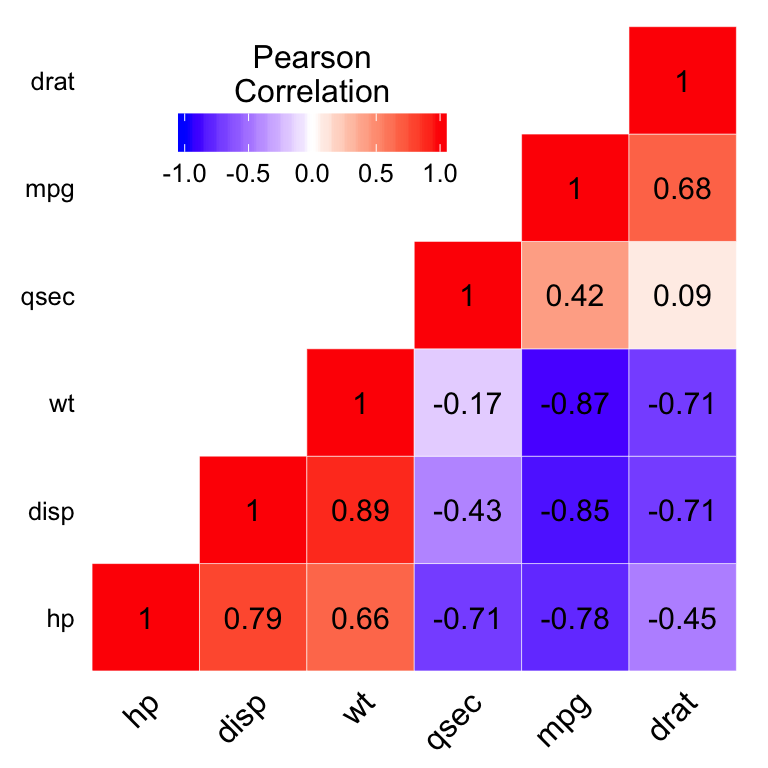
\includegraphics[scale=0.3]{heatmap.png}}
	\caption{Exemplo de Heat Map com matriz}
	\label{figura:heatmap}
\end{figure}

Será utilizado um gráfico de duas dimensões para mostrar a evolução das métricas ao longo do tempo como mostra as figura 3.4. O eixo x do gráfico representa o tempo e o eixo y representa o valor da métricas, sendo que o tempo está dividido a cada 15 dias.

\begin{figure}[H]
	\captionsetup{justification=centering}
	\centerline{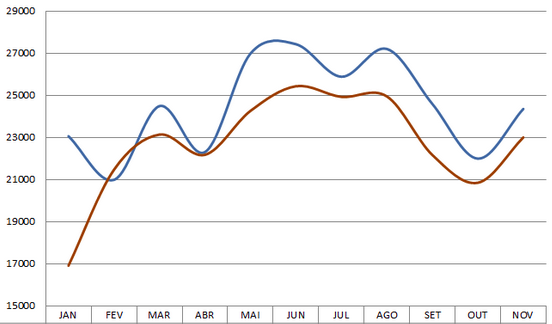
\includegraphics[scale=0.5]{metricaex.png}}
	\caption{Exemplo de gráfico de duas métricas ao longo do tempo}
	\label{figura:exmetrica}
\end{figure}

\section{Avaliar a ferramenta}
Para a avaliação, a ferramenta será configurada para 10 projetos e serão convidados desenvolvedores para utilizá-la. Os desenvolvedores deverão realizar tarefas sobre as funcionalidades da ferramenta, por exemplo, encontrar o valor da entropia em um determinado período de tempo no arquivo A, e após isso, responderão um questionário sobre a usabilidade da ferramenta. O questionário irá conter questões sobre a visualização de dados e o relatório estatístico para avaliar se a ferramenta auxilia o desenvolvedor na tomada de decisões do projeto.